%%%%%%%%%%%%%%%%%%%%%%%%%%%%%%%%%%%%%%%%%
% Arsclassica Article
% LaTeX Template
% Version 1.1 (10/6/14)
%
% This template has been downloaded from:
% http://www.LaTeXTemplates.com
%
% Original author:
% Lorenzo Pantieri (http://www.lorenzopantieri.net) with extensive modifications by:
% Vel (vel@latextemplates.com)
%
% License:
% CC BY-NC-SA 3.0 (http://creativecommons.org/licenses/by-nc-sa/3.0/)
%
%%%%%%%%%%%%%%%%%%%%%%%%%%%%%%%%%%%%%%%%%

%----------------------------------------------------------------------------------------
%	PACKAGES AND OTHER DOCUMENT CONFIGURATIONS
%----------------------------------------------------------------------------------------

\documentclass[
10pt, % Main document font size
a4paper, % Paper type, use 'letterpaper' for US Letter paper
oneside, % One page layout (no page indentation)
%twoside, % Two page layout (page indentation for binding and different headers)
headinclude,footinclude, % Extra spacing for the header and footer
BCOR5mm, % Binding correction
]{scrartcl}

%%%%%%%%%%%%%%%%%%%%%%%%%%%%%%%%%%%%%%%%%
% Arsclassica Article
% Structure Specification File
%
% This file has been downloaded from:
% http://www.LaTeXTemplates.com
%
% Original author:
% Lorenzo Pantieri (http://www.lorenzopantieri.net) with extensive modifications by:
% Vel (vel@latextemplates.com)
%
% License:
% CC BY-NC-SA 3.0 (http://creativecommons.org/licenses/by-nc-sa/3.0/)
%
%%%%%%%%%%%%%%%%%%%%%%%%%%%%%%%%%%%%%%%%%

%----------------------------------------------------------------------------------------
%	REQUIRED PACKAGES
%----------------------------------------------------------------------------------------

\usepackage[
nochapters, % Turn off chapters since this is an article        
beramono, % Use the Bera Mono font for monospaced text (\texttt)
eulermath,% Use the Euler font for mathematics
pdfspacing, % Makes use of pdftex’ letter spacing capabilities via the microtype package
dottedtoc % Dotted lines leading to the page numbers in the table of contents
]{classicthesis} % The layout is based on the Classic Thesis style

\usepackage{arsclassica} % Modifies the Classic Thesis package

\usepackage[T1]{fontenc} % Use 8-bit encoding that has 256 glyphs

\usepackage[utf8]{inputenc} % Required for including letters with accents

\usepackage{graphicx} % Required for including images
\graphicspath{{report_figures/}} % Set the default folder for images

\usepackage{enumitem} % Required for manipulating the whitespace between and within lists

\usepackage{lipsum} % Used for inserting dummy 'Lorem ipsum' text into the template

\usepackage{subfig} % Required for creating figures with multiple parts (subfigures)

\usepackage{amsmath,amssymb,amsthm} % For including math equations, theorems, symbols, etc

\usepackage{varioref} % More descriptive referencing

\usepackage[spanish]{babel} % Define spanish document
%----------------------------------------------------------------------------------------
%	THEOREM STYLES
%---------------------------------------------------------------------------------------

\theoremstyle{definition} % Define theorem styles here based on the definition style (used for definitions and examples)
\newtheorem{definition}{Definition}

\theoremstyle{plain} % Define theorem styles here based on the plain style (used for theorems, lemmas, propositions)
\newtheorem{theorem}{Theorem}

\theoremstyle{remark} % Define theorem styles here based on the remark style (used for remarks and notes)

%----------------------------------------------------------------------------------------
%	HYPERLINKS
%---------------------------------------------------------------------------------------

\hypersetup{
%draft, % Uncomment to remove all links (useful for printing in black and white)
colorlinks=true, breaklinks=true, bookmarks=true,bookmarksnumbered,
urlcolor=webbrown, linkcolor=RoyalBlue, citecolor=webgreen, % Link colors
pdftitle={}, % PDF title
pdfauthor={\textcopyright}, % PDF Author
pdfsubject={}, % PDF Subject
pdfkeywords={}, % PDF Keywords
pdfcreator={pdfLaTeX}, % PDF Creator
pdfproducer={LaTeX with hyperref and ClassicThesis} % PDF producer
}
 % Include the structure.tex file which specified the document structure and layout

\hyphenation{Fortran hy-phen-ation} % Specify custom hyphenation points in words with dashes where you would like hyphenation to occur, or alternatively, don't put any dashes in a word to stop hyphenation altogether

%----------------------------------------------------------------------------------------
%	TITLE AND AUTHOR(S)
%----------------------------------------------------------------------------------------

\title{\normalfont\spacedallcaps{Lenguajes para el desarrollo de aplicaciones móviles}} % The article title

\author{\spacedlowsmallcaps{Diego Trabazo Sardón* 
\& Raul Santoveña Gómez\textsuperscript{1}}} % The article author(s) - author
% affiliations need to be specified in the AUTHOR AFFILIATIONS block

\date{\today} % An optional date to appear under the author(s)
\setlength{\parskip}{1em}
%----------------------------------------------------------------------------------------

\begin{document}

%----------------------------------------------------------------------------------------
%	HEADERS
%----------------------------------------------------------------------------------------

\renewcommand{\sectionmark}[1]{\markright{\spacedlowsmallcaps{#1}}} % The header for all pages (oneside) or for even pages (twoside)
%\renewcommand{\subsectionmark}[1]{\markright{\thesubsection~#1}} % Uncomment when using the twoside option - this modifies the header on odd pages
\lehead{\mbox{\llap{\small\thepage\kern1em\color{halfgray} \vline}\color{halfgray}\hspace{0.5em}\rightmark\hfil}} % The header style

\pagestyle{scrheadings} % Enable the headers specified in this block

%----------------------------------------------------------------------------------------
%	TABLE OF CONTENTS & LISTS OF FIGURES AND TABLES
%----------------------------------------------------------------------------------------

\maketitle % Print the title/author/date block

\setcounter{tocdepth}{2} % Set the depth of the table of contents to show sections and subsections only

\tableofcontents % Print the table of contents

%\listoffigures % Print the list of figures

%\listoftables % Print the list of tables

%----------------------------------------------------------------------------------------
%	ABSTRACT
%----------------------------------------------------------------------------------------
\begin{abstract}
Desde el comienzo de los tiempos de la informática la búsqueda de sistemas físicamente más pequeños ha sido incesante. Hoy en día disponemos de dispositivos que caben en un bolsillo y gracias a la energía suministrada por baterías ofrecen a sus usuarios horas de autonomía y ofrecen multitud de servicios. Existe por supuesto un mercado de software muy activo que explota sus características. Con tantas opciones y fabricantes como hay en la actualidad para los clientes, no menos grande es el abanico para los desarrolladores. Una amplia variedad de lenguajes y sistema operativos pueden ser tenidos en cuenta. Se tratan en este documento la plataforma Android utilizando Java y Código Nativo. Además también se explica el uso de los lenguajes de la Web, HTML, CSS y JavaScript a la hora de crear una buena experiencia de usuario.
\end{abstract}


%----------------------------------------------------------------------------------------
%	AUTHOR AFFILIATIONS
%----------------------------------------------------------------------------------------

{\let\thefootnote\relax\footnotetext{* \textit{diego.trabazo@udc.es, Facultad de Informática, UDC}}}

{\let\thefootnote\relax\footnotetext{\textsuperscript{1} \textit{Department of Chemistry, University of Examples, London, United Kingdom}}}

%----------------------------------------------------------------------------------------

\newpage % Start the article content on the second page, remove this if you have a longer abstract that goes onto the second page

%----------------------------------------------------------------------------------------
%	INTRODUCTION
%----------------------------------------------------------------------------------------
\section{Introducción}
El sector de los dispositivos móviles ha crecido de manera muy relevante desde el 2007. No es que antes de esa fecha no hubiese computadoras de pequeño tamaño que incorporasen una batería como fuente de energía principal, una pantalla que sirviese de forma de entrada de información, y no sólo para mostrarla como en un ordenador; o interfaces de usuario distintas al teclado y ratón. Pero en el 2007 Apple dio a conocer el primer smartphone de pantalla táctil \cite{rob_price_how_2015} y varias de sus características cambiaron el mercado. Primero la posibilidad de ser utilizado para visualizar imágenes, vídeos, juegos u otro contenido multimedia. La creación de una tienda de aplicaciones que podían ser escritas por terceros desarrolladores, no sólo por Apple. Y por último estos teléfonos se acompañaban de una tarifa de datos, lo cual hizo que Internet estuviese disponible en todo momento. En el 2010, nuevamente Apple, presentó el iPad \cite{john_d._sutter_apple_2010}, que amplió la pantalla hasta convertirse en un dispositivo muy apropiado para el consumo multimedia.

Hoy en día hay muchas alternativas a la hora de adquirir un teléfono o tableta, pero además el modelo se ha extendido a nuevos productos como los relojes o \textit{smartwatches} o los coches con sistemas de \textit{infotainment}. El software utilizado en estos nuevos dispositivos es una adaptación de los sistemas Android o iOS existentes para estos nuevos formatos. Entre sus características comunes están que el método de entrada principal son o bien la voz o bien los gestos sobre la pantalla. Además son dependientes de un teléfono con el que suelen tener que estar emparejados.

\begin{figure}[h]
\centering 
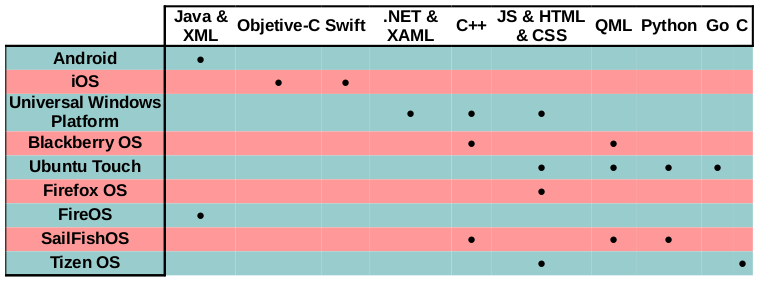
\includegraphics[width=1.1\columnwidth]{report_table_os_lang} 
\caption[Lenguajes recomendados por cada plataforma]{Lenguajes de programación recomendados por cada plataforma.} 
\label{fig:os_lang} 
\end{figure}

Para hacerse una idea de qué lenguajes se pueden utilizar en cuál plataforma basta mirar la figura \vref{fig:os_lang} que refleja las opciones recomendadas por el desarrollador de cada plataforma. No pretende ser exhaustiva, pero si dar una idea de que es lo recomendado. Mencionar de forma especial, ya que llama la atención, que en Tizen las aplicaciones nativas se escriban en lenguaje C. No se esperaba a priori que se hiciese uso de lenguajes no Orientados a Objetos para el desarrollo de aplicaciones. Téngase en cuenta que las interfaces de usuario siguen el paradigma de la Orientación a Eventos. El desarrollador define métodos Callback que son llamados por el sistema o por otros métodos de la aplicación de forma automática ante una circunstancia determinada.

%----------------------------------------------------------------------------------------
%	HTML
%----------------------------------------------------------------------------------------
\section{Html: ¿multiplataforma?}
Una opción a considerar a la hora de desarrollar aplicaciones Web modernas es el conjunto de lenguajes habituales de la Web: Html 5, CSS y JavaScript. Es posible construir y distribuir aplicaciones usando estos tres lenguajes pero hay una serie de aspectos, que se verán a continuación y que conviene tener en cuenta. Los objetivos que se suelen perseguir con este enfoque son tanto económicos como tecnológicos: 

\begin{itemize}
\item Disponibilidad multiplataforma: Una misma aplicación debería poder funcionar el todas las plataformas en las que la empresa quiera estar presente.
\item Aprovechamiento de los conocimientos de los desarrolladores existentes en la organización para abarcar un ámbito nuevo y diferente a la Web tradicional.
\item Aprovechar el esfuerzo ya realizado cuando se creó la web de la organización.
\end{itemize}

Los principio de separación de aspecto y comportamiento siguen siendo primordiales en la Web de hoy en día con HTML 5 y CSS 3. El primero es un lenguaje de marcado cuya principal misión es crear la estructura donde los elementos de la web tienen que ser colocados. Se dota al contenido de contexto, quedando claro que es cada elemento. Con CSS se trabaja todo lo relativo al aspecto final: colores, fuentes o tipografías, maquetación. Un concepto central a CSS es el \textit{Box Model} que agrupa los elementos de la página dentro de cajas que se pueden colocar de distintas maneras o se pueden comportar de distintas maneras dependiendo del dispositivo de visualización.

\subsection{1ª aproximación: WebView / UIWebView / WebBrowser}
En primer lugar y de manera básica, todas las plataformas disponen de algún \textit{browser engine} del cual el programador puede aprovecharse para mostrar contenido web correctamente adaptado a las características de la pantalla del dispositivo, estas son, como mínimo, tamaño y orientación. Esto quiere decir que usando las propias características del lenguaje HTML y haciendo uso de Responsive Web Design, se pueden crear sitios web que cumplan con los objetivos de poner al alcance del usuario final los contenidos o herramientas de la web de la empresa u organización en un formato manejable. No obstante esta aproximación puede no ser suficiente en muchos casos y dista bastante de ser una aplicación móvil como tal. No obstante, a día de hoy las APIs disponibles dan muchas posibilidades. Sólo por citar algunas áreas, 

\begin{itemize}[noitemsep]
\item Vídeo a pantalla completa con subtítulos si se desea.
\item Funciones de localización geográfica.
\item Funcionalidad offline.
\item Almacenamiento y consultas en bases de datos.
\item Notificaciones integradas con el sistema.
\item Manipulación de recursos JSON.
\item WebGL para contenido en 3D.
\item WebWorkers para ejecución con threads.
\item y mucho más... \cite{mozilla_developer_network_web_2016}
\end{itemize}

\subsection{Safari, Chrome, y Windows apps}
No obstante a lo dicho anteriormente para conseguir una mayor integración con cada plataforma y que el usuario disfrute de la misma experiencia hacen falta más cosas. Principalmente 

\begin{enumerate}
\item Poder especificar que la página web disponga de su propio icono en la \textit{home screen} del dispositivo.
\item Posibilidad de compartir contenido entre aplicaciones instaladas en el dispositivo.
\item Cambiar la apariencia (por ejemplo los colores) de las barras de estado.
\item Disponer de una imagen de inicio (mayoritariamente en iOS).
\end{enumerate}

Hay que tener en cuenta que no todos los navegadores soportan las mismas características ni las implementaciones existentes son las mismas. Baste como ejemplo el caso de la \textit{Vibration API} estaba soportada por Chrome en su versión 40b sobre Android 4.0 pero que es inexistente en iOS y Windows, como se puede ver en \cite{mozilla_developer_network_web_2016}.

\subsection{APIs nativas}
Si se desea mayor integración con la plataforma o mejorar el rendimiento, se puede hacer uso de las APIs nativas desde JavaScript. Para un desarrollo profesional se puede recurrir a alguno de los muchos Frameworks existentes. No proveen tanto un nuevo lenguaje de programación sino más bien un conjunto de librerías intermedias que homogeinizan el desarrollo. Por ejemplo PhoneGap \cite{adobe_systems_inc._phonegap_2016}, que utiliza internamente el framework Cordova \cite{the_apache_software_foundation_apache_2016} permite el desarrollo de una única aplicación que genera ejecutables para iOS, Android o Windows. Todo de forma transparente para el usuario. Además esta plataforma también ofrece infraestructura para realizar compilación y empaquetado.
Otro caso es el de Ionic \cite{drifty_co._building_2016}. Ionic mejora la apariencia de las aplicaciones acercándolas más a las nativas de la plataforma \cite{kacie_clark_introduction_2015}

%----------------------------------------------------------------------------------------
%	JAVA EN ANDROID
%----------------------------------------------------------------------------------------
\section{Android}
Android es un sistema operativo desarrollado por Google, basado en Linux y diseñado principalmente para dispositivos móviles con pantalla táctil como smartphones y tabletas. Además de los dispositivos táctiles, Google ha desarrollado Android TV para televisiones, Android Auto para automóviles, y Android Wear para relojes, cada uno con sus peculiaridades. También existen variantes de Android usadas en ordenadores, videoconsolas, cámaras digitales, y otros aparatos electrónicos.

\subsection{Un poco de historia}
Su nacimiento y desarrollo, fue obra de la compañía Android Inc., que fue financiada inicialmente por Google, para ser comprada posteriormente por esta misma, en el año 2005. En 2007, Google da a conocer oficialmente su SO Android, presentando la primera versión llamada Android 1.0 Apple Pie. Pero no sería hasta finales del 2008, cuando de manos del HTC Dream, vería la luz de cara al público. 

En 2013 las encuestas situaban a Android como el dominante en el desarrollo de aplicaciones móviles, con un 71\% de los desarrolladores creando sus aplicaciones para el sistema operativo de Google. En septiembre de 2015, en la calle había ya 1.4 billones de dispositivos móviles activos funcionando con Android. Actualmente, datos del primer trimestre de 2016 sitúan a Android con una cuota de mercado del 84.1\%.

Como curiosidad, en un principio, Android fue ideado como un sistema operativo para usar con teclado y cursor para poder navegar entre aplicaciones. Más tarde, antes de que se lanzara el primer dispositivo Android, la filosofía cambió para convertirse en un sistema operativo orientado a los dispositivos táctiles, para así competir contra el iPhone de Apple, presentado 1 año y 9 meses antes.

\subsection{Desarrollo de aplicaciones para Android}
Normalmente, para el desarrollo de aplicaciones en Android, se utiliza Java, lenguaje de programación de propósito general, concurrente y orientado a objetos. Su sintaxis deriva en gran medida de C y C++, pero tiene menos utilidades de bajo nivel que cualquiera de ellos. Las aplicaciones de Java son generalmente compiladas a bytecode (clase Java) que puede ejecutarse en cualquier máquina virtual Java (JVM). En el caso de Android, hay pequeñas variaciones. Aunque la mayoria de las apps están escritas en Java, no hay una máquina virtual Java, el bytecode Java no es ejecutado, sino que se compila en lo que se conoce como Dalvik ejecutable (una traducción de Java bytecode) y se ejecuta en la Máquina Virtual Dalvik, máquina virtual diseñada especificamente para Android. La máquina virtual Dalvik estuvo presente hasta la versión 5.0 de Android, ya que a partir de la versión de 4.4 se introdujo ART (Android Runtime), un nuevo entorno de ejecución, que compila el Java bytecode durante la instalación de la aplicación. Ambas versiones estuvieron coexistiendo un tiempo, dandole la posibilidad al usuario del dispositivo móvil de escoger entre las dos. Con la versión 5.0, esta opción desapareció y ART quedó como la única opción. Aunque Java utiliza el paradigma orientado a objetos, es importante remarcar que Android se basa en la filosofia orientada a eventos. Es decir, en una aplicación Android se recogen eventos generados bien por el sistema, bien por otras aplicaciones, o bien por el usuario. Por lo tanto, no existe un main donde la aplicación comienza a ejecutarse, sino que surgen eventos a los que la aplicación reacciona ejecutando el código oportuno.  A mayores, Google proporciona un kit de desarrollo software más conocido como SDK de Android, que proporciona un conjunto de herramientas de desarrollo. El SDK está formado por un depurador de código, bibliotecas, un simulador de un telefono Android, documentación, ejemplos de código y tutoriales. El IDE oficial es Android Studio, aunque también pueden utilizarse otros IDEs como Eclipse mediante plugins, aunque esta opción ha ido perdiendo fuerza y usuarios conforme Google ha ido actualizando y mejorando Android Studio. El SDK de Android es soportado en diversas plataformas, como Linux, Mac OS X, Windows e incluso el propio Android.

Para iniciarse en el desarrollo de aplicaciones en Android tan sólo se requieren unos conocimientos aceptables de programación y un conocimiento básico de Java para su uso, amén del SDK, herramienta que puede descargarse de manera gratuita, por lo que el coste para realizar una aplicación Android es nulo. A la hora de publicar una aplicación en la Play Store de Google es necesario crear una cuenta de desarrollador y abonar una única cuota para el alta de 25\$, sin más cuotas posteriores. Si la aplicación publicada generase beneficios al desarrollador o desarrolladores, Google se queda con el 30\% y el desarrollador recibe el 70\%.

Pero desarrollar aplicaciones Android por medio de Java y del kit de desarrollo software de Google no es la única alternativa. Entre las propias herramientas oficiales que Google proporciona para trabajar en Android se encuentra el NDK (Native Development Kit), un kit de desarrollo nativo que como su nombre indica permite incorporar código nativo en C o C++ en aplicaciones Android, aunque sólo debería usarse cuando sea estrictamente necesario, y no simplemente porque el programador prefiera lenguajes como C++ o C, ya que su uso aumenta considerablemente la complejidad del código. Además, existen innumerables herramientas de desarrollo de terceros que nos permiten trabajar y programar en otros lenguajes como por ejemplo App Inventor, entorno visual para programadores novatos y varios marcos de aplicaciones basadas en la web multiteléfono. 

La ventaja de trabajar con un lenguaje nativo como Java en Android es que podemos aprovecharlo para sacar el máximo rendimiento a los dispositivos que cuenten con este sistema operativo. Además, la documentación aportada por Google para programar en Android utilizando Java y el kit de desarrollo oficial es muy extensa y está en continua actualización. De estas ventajas, deriva una tercera, ya que dada la relativa facilidad que supone empezar a crear aplicaciones Android con las herramientas de Google, se ha creado una gran comunidad programando apps en Android de esta manera, por lo tanto la comunidad de usuarios que tiene detrás y que puede proporcionar ayuda ante todo tipo de problemas es enorme.

A pesar de las ventajas que pueda suponer utilizar las herramientas nativas, es interesante echar un vistazo a la distintas alternativas que pueden encontrarse, por lo que en las siguientes lineas se comentarán brevemente algunas herramientas y que ventajas pueden aportar frente a Java y el SDK de Android.

\begin{itemize}
	\item App Inventor: Herramienta desarrollada para programar en Android de manera sencilla orientada a programadores principiantes. Se basa en un entorno totalmente visual, sin código de por medio, donde el usuario puede ir enlazando una serie de bloques para crear la aplicación. Esta simplicidad permite a usuarios sin conocimientos de programación la posibilidad de realizar aplicaciones en Android, sin utilizar lenguajes de programación, pero también limita muchos las posibilidades de creación, siendo esta su mayor desventaja.

	\item El proyecto Simple: Simple es un dialecto de BASIC para Android. Orientado a programadores aficionados, pero no limitado a ellos, permite escribir rápidamente aplicaciones que utilizan los componentes de ejecución de Android. El objetivo de Simple es ser un lenguaje fácil de aprender.

	Parecido a Visual Basic 6 de Microsoft, los programas Simple consisten en definiciones de formularios (que contienen componentes) y código (con la lógica del programa). La interacción entre ellos se hace por medio de eventos lanzados por los componentes. La lógica del programa consiste en gestores de eventos, que ejecutan código dependiendo del evento.

	El proyecto Simple no tiene mucha actividad. La última actualización de código se realizó en agosto de 2009.

	\item Basic4android: Proyecto similar a Simple, inspirado en Microsoft Visual Basic 6 y Microsoft Visual Studio, Basic4Android es una plataforma que facilita la creación de aplicaciones Android para programadores habituales de Visual Basic. Entre sus ventajas, destaca un entorno más gráfico y menos abstracto, especialmente indicado para desarrolladores nóveles en Android.

	\item HyperNext Android Creator: Sistema para el desarrollo de aplicaciones dirigido a programadores junior, que permite crear aplicaciones sin conocimientos de Java ni del SDK de Android. Está basado en HyperCard, una aplicación informatica de Apple Computer, que se basa en el concepto de una pila de tarjetas virtuales, en la que sólo una de ellas es visible en un momento dado, concepto similar al utilizado en aplicaciones para teléfonos móviles, con una sola ventana disponible a la vez. El lenguaje utilizado por HyperNext Android Creator es HyperNext, y recoge ideas del lenguaje utilizado en HyperCards llamado HyperTalk. HyperNext posee muchas funciones para crear aplicaciones Android, soportando muchas funcionalidades del SDK de Android.

	\item Processing: Permite crear aplicaciones Android para smartphones, tablets o smartwatches con pocos o ningún cambio en el código y sin tener que ocuparse de tareas como instalar archivos SDK, crear carpetas de proyectos o editar archivos de diseño. También permite acceder a las funcionalidades del SDK de Android para obtener acceso a sensores y otras funciones avanzadas.

	\item Qt para Android: Qt para Android permite a las aplicaciones Qt 5 funcionar en dispositivos Android V2.3.3 ( nivel de API 10) o posteriores. Qt es una infraestructura multiplataforma para aplicaciones de todo tipo, entre ellas aplicaciones móviles, por lo que daremos más detalles sobre ella en el tema de de desarrollo multiplataforma.

	\item RFO Basic!: RFO Basic es un dialecto del lenguaje Basic Dartmouth, versión original del lenguaje de programación BASIC, que proporciona acceso a hardware, sensores, sonido, gráficos, funciones multitactil, sistema de ficheros, SQLite, sockets, FTP, HTTP, Bluetooth, HTML GUI, encryption, SMS, teléfono, correo, texto a voz, reconocimiento de voz, GPS, funciones matemáticas, funciones de cadenas de caracteres, listas y otras utilidades esenciales. Permite escribir y ejecutar programas directamente en un dispositivo Android. Es un proyecto de código abierto que produce ficheros apk de Android independientes. Su desarrollo está activo y tiene una fuerte comunidad en línea de desarrolladores.

	\item Ruboto: Framework y conjunto de herramientas para desarrollar aplicaciones nativas en Android utilizando el lenguaje Ruby. Las aplicaciones creadas con Ruboto pueden ser desarrolladas usando JRuby, MRI o Rubinius. Las aplicaciones creadas dependen de JRuby (jruby-jars) en tiempo de ejecución para proporcionar acceso completo a las API Java de Android. Posee bastante documentación para empezar a programar.
\end{itemize}

Uno de los denominadores comunes entre casi todas las herramientas mencionadas, es la intención de simplificar el desarrollo de las aplicaciones, ya que en algunos casos puede volverse un tanto difícil el uso de las herramientas nativas. Esta característica es una ventaja para aquellos que quieren iniciarse en el desarrollo móvil o que aún no poseen muchas nociones de programación, o para los que tan solo desean realizar aplicaciones no demasiado complejas. Pero es a la vez su punto débil, ya que a la hora de desarrollar aplicaciones avanzadas, la mayoría de estas herramientas seguramente se quedarían cortas para poder desarrollar todas las funcionalidades deseadas. Otra posible ventaja, es que emplean diferentes lenguajes, que podrían permitir al usuario programar aplicaciones Android en lenguajes que ya conozca sin tener que adentrarse en el aprendizaje de un nuevo lenguaje, algo que muchas veces frena a los desarrolladores a la hora de trabajar en un nuevo sistema operativo.

Existen muchas otras plataformas que permiten la programación en Android abstrayéndonos en muchas ocasiones de Java y de las herramientas de desarrollo de Google, algunas de ellas multiplaforma, es decir, no solo nos permiten programar aplicaciones Android, sino aplicaciones que funcionen también en otros sistemas operativos como puede ser iOS o Windows Phone entre otros. En un tema venidero abordaremos esta temática por lo que se ha decidido no comentarlas como un uso específico para Android y sí hablar de una manera mas genérica llegado el momento.


%----------------------------------------------------------------------------------------
%	DESARROLLO MULTIPLAFORMA
%----------------------------------------------------------------------------------------
\section{Desarrollo multiplataforma}
Una opción para el desarrollo de aplicaciones móviles es utilizar alguna plataforma que independice el desarrollo del lenguaje nativo de cada plataforma móvil. Con el uso de estas herramientas se utiliza un único lenguaje y se crean aplicaciones que funcionan en varias plataformas, eso sí, adaptando algunas cuestiones para que las aplicaciones puedan funcionar en cada caso. La mayor ventaja de estas herramientas es que permiten programar en un solo lenguaje, se reutiliza la mayoría del código entre todas las plataformas, y además se generan aplicaciones nativas para los entornos móviles de los que disponen.

\begin{itemize}
	\item Xamarin: Basada en el lenguaje C\# de Microsoft y en la plataforma .NET, gracias a sus herramientas permite crear aplicaciones para plataformas como iOs, Android y Windows Phone entre otras, reutilizando gran parte del código (a excepción de la interfaz).

	Las aplicaciones escritas con Xamarin en C\# se compilan a código nativo en cada plataforma, por lo que su rendimiento es exactamente el mismo que el de una aplicación nativa. Además ofrece acceso directo nativo a todas las APIs de cada plataforma así como a los controles de interfaz de usuario nativos, de hecho esto último es lo que debes aprender con Xamarin para cada plataforma de manera diferente según quieras programar para iOS, Android o Windows Phone.

	\item LiveCode: LiveCode es una aplicación multiplataforma que permite desarrollar programas que funcionen no solo en dispositivos móviles con iOS o Android, sino que permite desarrollar también ese mismo programa para Windows, LINUX, MacOSX, etc...

	LiveCode está inspirado en el lenguaje HyperTalk, ya mencionado anteriormente. Es un lenguaje bastante sencillo, similar al inglés. Cuenta con aproximadamente 1900 sentencias de programación, aunque pueden ampliarse utilizando plugins o programando en C. La idea del funcionamiento de la herramienta puede verse como la de una baraja de cartas, que se denominaria "Main Stack", de la cual cuelgan cartas. Estas cartas se corresponden con lo que son las pantallas de una aplicación, siendo su funcionamiento parecido al de Visual Basic.

	A pesar de los beneficios que puede llegar a proporcionar, también presenta problemas. La flexibilidad a la hora de desarrollar para multiples plataformas también provoca que estas no puedan explotarse al máximo y no puedan ejecutarse algunas de sus funcionalidades. No existe demasiada documentación y la comunidad de usuarios no es excesivamente grande. Además, hay comandos de la aplicación que no funcionan en todas las plataformas.

	\item HTML5: Lenguaje que posee una gran versatilidad con lo que permite adaptarse a muchas plataformas, es probablemente el lenguaje ideal para el desarrollo multiplataforma, y es utilizado además en diversas plataformas móviles como por ejemplo en Firefox OS. Por su importancia, ha decidido dedicarse un apartado exclusivo que abordará más en detalle este lenguaje.

	\item Kivy: Kivy es una librería escrita en Python de código abierto que proporciona funcionalidades para desarrollar apps para móviles y otras aplicaciones informáticas multitáctiles. Utiliza una interfaz natural de usuario (NUI), y puede utilizarse para crear aplicaciones que corran en Android, iOS, Linux, OS X y Windows. Tiene una herramienta incorporada para distribuir aplicaciones móviles llamada Buildozer, sólo disponible en Linux. 

	\item Qt: Qt es una infraestructura multiplataforma de código abierto para  aplicaciones que puede abarcar a Android, Linux, iOS, Sailfish OS, Windows e incluso sistemas empotrados. Utiliza el lenguaje C++ de forma nativa, aunque pueden utilizarse otros lenguajes de programación a través de bindings. Proporciona un entorno de desarrollo integrado llamado Qt Creator. Para el desarrollo de aplicaciones en Android, es necesario tanto el NDK como JDK.

	\item RubyMotion: RubyMotion es una herramienta para desarrollar aplicaciones móviles multiplataforma utilizando el lenguaje Ruby. Permite crear aplicaciones nativas en Android, iOS y OS X. Un ejemplo de aplicación desarrollada con esta herramienta es A Dark Room, un juego de rol basado en texto originalmente creado para web, y que fue portado a iOs mediante RubyMotion.

	\item SDL: Simple DirectMedia Layer (SDL) es una libreria escrita en C para desarrollo multiplataforma que proporciona funcionalidades de bajo nivel para acceso a audio, teclado, ratón, joystick y gráficos a través de OpenGL y Direct3D. 

	Es utilizado en software de reproducción de vídeo, emuladores y videojuegos. SDL admite oficialmente Windows, Mac OS X, Linux, iOS y Android. Aunque puede encontrarse soporte para más plataformas.

	SDL está escrito en C, funciona de forma nativa con C++, y hay bindings disponibles para muchos otros lenguajes, como C\#, Python, Ada, BASIC, Erlan, Lua, Java o Python entre otros.

	\item WinDev Mobile: WinDev Mobile  permite crear potentes aplicaciones para smartphones y tablets. Soporta Android, iOS, Windows 10 Mobiles, CE, etc... Utiliza WLanguage como lenguaje de programación, un lenguaje simple y flexible, cercano al lenguaje natural.

	\item Appcelerator Titanium: Framework de código abierto que permite crear aplicaciones móviles para Android, iOS y Windows Phone utilizando Javascript. El componente principal del framework es el Titanium SDK, liberado bajo licencia Apache. Cuenta con aproximadamente 900.000 desarrolladores registrados. Existe mucha documentación e incluso es utilizado por grandes empresas para desarrollar sus aplicaciones.

	\item RhoMobile Suite: RhoMobile Suite es un conjunto de herramientas de desarrollo para crear aplicaciones móviles nativas y multiplataforma. Está basado en el framework de código abierto Rhodes. RhoMobile permite construir aplicaciones móviles nativas usando tecnologías web, como CSS3, HTML5, JavaScript y Ruby. A través del software proporcionado por RhoMobile se puede escribir una aplicación un única vez y hacer que corra en distintos sistemas operativos como iOS, Android, Windows Phone, Windows CE, Blackberry, etc... Pudiendo controlar como las aplicaciones se comportan en los distintos dispositivos. RhoMobile Suite está formado por un conjunto de herramientas para construir, probar, depurar, integrar, desplegar y gestionar las aplicaciones. Para proporcionar todas estas funcionalidades RhoMobile Suite se divide en distintos productos:
	\begin{itemize}
		\item RhoStudio:  potente plug-in para Eclipse que permite desarrollar, probar y depurar las aplicaciones, incluye RhoSimulator, un dispositivo y simulador de plataforma personalizado para el desarrollo de las aplicaciones RhoMobile.

		\item RhoMobile: contender de las aplicaciones móviles que se ejecuta como una aplicación nativa, pero permite escribir fácilmente código multiplataforma utilizando un punto de vista más cercano al desarrollo web. Soporta lenguajes estándar como JavaScript, HTML, CSS y Ruby. RhoMobile proporciona acceso al dispositivo, su sistema y el framework a través de sus librerias Rhodes y RhoElements
		\begin{itemize}
			\item Rhodes: es un conjunto de librerías de código abierto accesibles para todas las aplicaciones RhoMobile. Proporciona acceso a través de interfaces JavaScript y Ruby. Permite acceder a funcionalidade como la cámara del dispositivo o el GPS.
			\item RhoElements: conjunto adicional de librerías, al igual que Rhodes, están escritas en Javascript y Ruby. A diferencia de Rhodes, RhoElements proporciona funcionalidades a nivel empresarial.
		\end{itemize}

		\item RhoConnect: servidor de aplicaciones que entre otras cosas permite conectarse a diferentes fuentes de datos como servicios web, bases de datos, etc...

	\end{itemize}
	Entre sus ventajas, destacar que permite incluir el uso de hardware integrado en el dispositivo, permitiendo el acceso a la cámara o al GPS por ejemplo, y además, de una manera relativamente sencilla. También permite aplicar el patrón MVC para facilitar el desarrollo.
\end{itemize} 

Las principales ventajas de las herramientas multiplataforma es que permiten programar en un solo lenguaje, pudiendo escoger una herramienta cuyo lenguaje ya domines, y así evitar el aprendizaje de un nuevo lenguaje. Las aplicaciones creadas funcionaran en varias plataformas, tantas como la herramienta soporte, por lo que acortan el tiempo de desarrollo, ya que idealmente, sólo es necesario un único desarrollo, y no uno para cada plataforma, por lo que se produce un ahorro en tiempo y coste. Por otro lado, estas herramientas también tienen sus inconvenientes. Se añade una capa de abstracción al desarrollo de la aplicación por lo que la capacidad para poder aprovechar todas las funcionalidades que presente la plataforma se limita. Por este mismo motivo, la capacidad de optimización es practicamente nula, ya que cada sistema operativo tiene sus caracteristicas y si se programa una aplicación que tiene que funcionar en todos es imposible aplicar optimizaciones especificas para el sistema que mejoren el rendimiento, los desarrolladores trabajan en lenguajes que no son nativos para las plataformas; por eso, la eficacia del código depende del motor de traducción. Sucede a menudo que las técnicas de codificación son ineficientes o que el código es redundante.


% A statement\footnote{Example of a footnote} requiring citation \cite{Figueredo:2009dg}.
% 
% \lipsum[1-3] % Dummy text
% 
% Some mathematics in the text: $\cos\pi=-1$ and $\alpha$.
%  
% %----------------------------------------------------------------------------------------
% %	METHODS
% %----------------------------------------------------------------------------------------
% 
% \section{Methods}
% 
% Reference to Figure~\vref{fig:gallery}. % The \vref command specifies the location of the reference
% 
% \begin{figure}[tb]
% \centering 
% 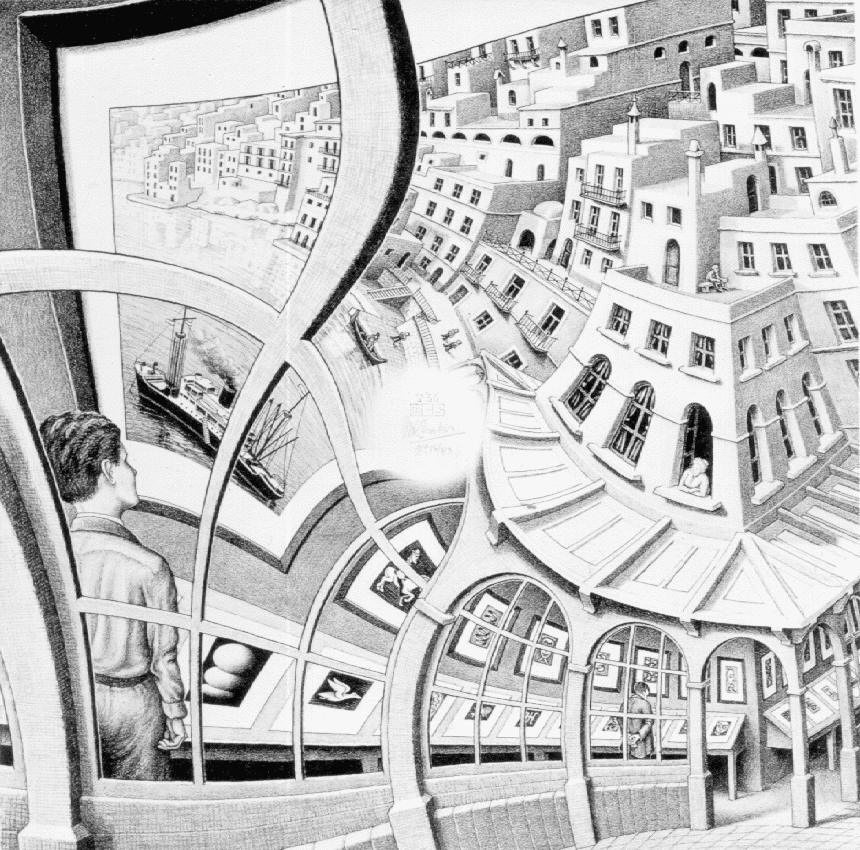
\includegraphics[width=0.5\columnwidth]{GalleriaStampe} 
% \caption[An example of a floating figure]{An example of a floating figure (a reproduction from the \emph{Gallery of prints}, M.~Escher,\index{Escher, M.~C.} from \url{http://www.mcescher.com/}).} % The text in the square bracket is the caption for the list of figures while the text in the curly brackets is the figure caption
% \label{fig:gallery} 
% \end{figure}
% 
% \lipsum[5] % Dummy text
% 
% \begin{enumerate}[noitemsep] % [noitemsep] removes whitespace between the items for a compact look
% \item First item in a list
% \item Second item in a list
% \item Third item in a list
% \end{enumerate}
% 
% %------------------------------------------------
% 
% \subsection{Paragraphs}
% 
% \lipsum[6] % Dummy text
% 
% \paragraph{Paragraph Description} \lipsum[7] % Dummy text
% 
% \paragraph{Different Paragraph Description} \lipsum[8] % Dummy text
% 
% %------------------------------------------------
% 
% \subsection{Math}
% 
% \lipsum[4] % Dummy text
% 
% \begin{equation}
% \cos^3 \theta =\frac{1}{4}\cos\theta+\frac{3}{4}\cos 3\theta
% \label{eq:refname2}
% \end{equation}
% 
% \lipsum[5] % Dummy text
% 
% \begin{definition}[Gauss] 
% To a mathematician it is obvious that
% $\int_{-\infty}^{+\infty}
% e^{-x^2}\,dx=\sqrt{\pi}$. 
% \end{definition} 
% 
% \begin{theorem}[Pythagoras]
% The square of the hypotenuse (the side opposite the right angle) is equal to the sum of the squares of the other two sides.
% \end{theorem}
% 
% \begin{proof} 
% We have that $\log(1)^2 = 2\log(1)$.
% But we also have that $\log(-1)^2=\log(1)=0$.
% Then $2\log(-1)=0$, from which the proof.
% \end{proof}
% 
% %----------------------------------------------------------------------------------------
% %	RESULTS AND DISCUSSION
% %----------------------------------------------------------------------------------------
% 
% \section{Results and Discussion}
% 
% \lipsum[10] % Dummy text
% 
% %------------------------------------------------
% 
% \subsection{Subsection}
% 
% \lipsum[11] % Dummy text
% 
% \subsubsection{Subsubsection}
% 
% \lipsum[12] % Dummy text
% 
% \begin{description}
% \item[Word] Definition
% \item[Concept] Explanation
% \item[Idea] Text
% \end{description}
% 
% \lipsum[12] % Dummy text
% 
% \begin{itemize}[noitemsep] % [noitemsep] removes whitespace between the items for a compact look
% \item First item in a list
% \item Second item in a list
% \item Third item in a list
% \end{itemize}
% 
% \subsubsection{Table}
% 
% \lipsum[13] % Dummy text
% 
% \begin{table}[hbt]
% \caption{Table of Grades}
% \centering
% \begin{tabular}{llr}
% \toprule
% \multicolumn{2}{c}{Name} \\
% \cmidrule(r){1-2}
% First name & Last Name & Grade \\
% \midrule
% John & Doe & $7.5$ \\
% Richard & Miles & $2$ \\
% \bottomrule
% \end{tabular}
% \label{tab:label}
% \end{table}
% 
% Reference to Table~\vref{tab:label}. % The \vref command specifies the location of the reference
% 
% %------------------------------------------------
% 
% \subsection{Figure Composed of Subfigures}
% 
% Reference the figure composed of multiple subfigures as Figure~\vref{fig:esempio}. Reference one of the subfigures as Figure~\vref{fig:ipsum}. % The \vref command specifies the location of the reference
% 
% \lipsum[15-18] % Dummy text
% 
% \begin{figure}[tb]
% \centering
% \subfloat[A city market.]{
\includegraphics[width=.45\columnwidth]{Lorem}} \quad
% \subfloat[Forest landscape.]{
\includegraphics[width=.45\columnwidth]{Ipsum}\label{fig:ipsum}} \\
% \subfloat[Mountain landscape.]{
\includegraphics[width=.45\columnwidth]{Dolor}} \quad
% \subfloat[A tile decoration.]{
\includegraphics[width=.45\columnwidth]{Sit}}
% \caption[A number of pictures.]{A number of pictures with no common theme.} % The text in the square bracket is the caption for the list of figures while the text in the curly brackets is the figure caption
% \label{fig:esempio}
% \end{figure}
% 

%----------------------------------------------------------------------------------------
%	BIBLIOGRAPHY
%----------------------------------------------------------------------------------------
\bibliographystyle{unsrt}

\bibliography{report_biblio.bib} % The file containing the bibliography

%----------------------------------------------------------------------------------------

\end{document}
